% Causal Parameters for Public Health Policy

\documentclass[aspectratio=169]{beamer}
\usetheme{Copenhagen}
\usecolortheme{whale}
\usefonttheme[onlymath]{serif}
\addtobeamertemplate{footnote}{\hskip -2em}{}

\usepackage{setspace}
\usepackage{xcolor}
\usepackage{graphicx}
\usepackage{multimedia}
\usepackage{fontawesome5}
\usepackage[most]{tcolorbox}
\usepackage{empheq}
\usepackage{fancybox}
\usepackage{annotate-equations}
\usepackage{soul}
\usepackage{tikz}
\usetikzlibrary{positioning, calc, shapes.geometric, shapes.multipart, 
	shapes, arrows.meta, arrows, 
	decorations.markings, external, trees}
\tikzstyle{Arrow} = [
thick, 
decoration={
	markings,
	mark=at position 1 with {
		\arrow[thick]{latex}
	}
}, 
shorten >= 3pt, preaction = {decorate}
]

\definecolor{teel}{HTML}{00AEB3}
\definecolor{redorange}{HTML}{F26035}
\definecolor{darkred}{HTML}{8B0000}
\definecolor{darkblue}{HTML}{00008B}
\definecolor{darkgreen}{HTML}{06402B}
\definecolor{CarolinaBlue}{HTML}{4B9CD3}
\definecolor{deepsea}{HTML}{123456}
\definecolor{sharedblue}{HTML}{009292}
\definecolor{distalblue}{HTML}{490092}

\usecolortheme[named=deepsea]{structure}

\title[Causal Parameters]{Causal Parameters for Public Health Policy}
\author[PN Zivich]{Paul Zivich \\ Assistant Professor \\ Department of Epidemiology \\ University of North Carolina at Chapel Hill}
\date{June 25, 2026}

\setbeamercovered{transparent}
\setbeamertemplate{navigation symbols}{}  % gets rid of the dumb navigation symbols
\setbeamertemplate{page number in head/foot}{\insertframenumber}  % adds slide #
\setbeamertemplate{headline}{}

\newcommand\blfootnote[1]{%
	\begingroup
	\renewcommand\thefootnote{}\footnote[frame]{#1}%
	\addtocounter{footnote}{-1}%
	\endgroup
}

\AtBeginSection[]{
	\begin{frame}
		\vfill
		\centering
		\begin{beamercolorbox}[sep=8pt,center,shadow=true,rounded=true]{title}
			\usebeamerfont{title}\insertsectionhead\par%
		\end{beamercolorbox}
		\vfill
	\end{frame}
}

\begin{document}
	
\begin{frame}[plain]
	\maketitle
\end{frame}

\begin{frame}{Acknowledgments\footnote[frame]{Footnotes are for asides or references}}
	\textbf{Funding}: K01AI177102
	~\\~\\
	\textbf{Conflicts of Interest}: None
	~\\~\\
	\textbf{Disclaimer}: All errors are my own
	~\\~\\
	\begin{center}
		\small
		\faEnvelope \quad pzivich@unc.edu \qquad \quad 
		\faGithub \quad pzivich \qquad \quad
		\faHashtag \quad pausalz@bsky.social
	\end{center}	
\end{frame}

\begin{frame}{Setup}
	\textbf{Notation}
	\begin{itemize}
		\item $Y$: outcome
		\item $A$: exposure
		\item $W$: additional baseline covariates
	\end{itemize}
	~\\
	\textbf{Perspective}: how the tools of causal inference can be used to help generate evidence for the impact of policies
	\begin{itemize}
		\item \textit{Policy}: rule or plan to modify $A$ for a defined group of people
		\item \textit{Policy Impact}: how the changes in $A$ modify $Y$ (intended or unintended)
	\end{itemize}
\end{frame}

\begin{frame}{Population Diagram Key}
	\begin{center}
		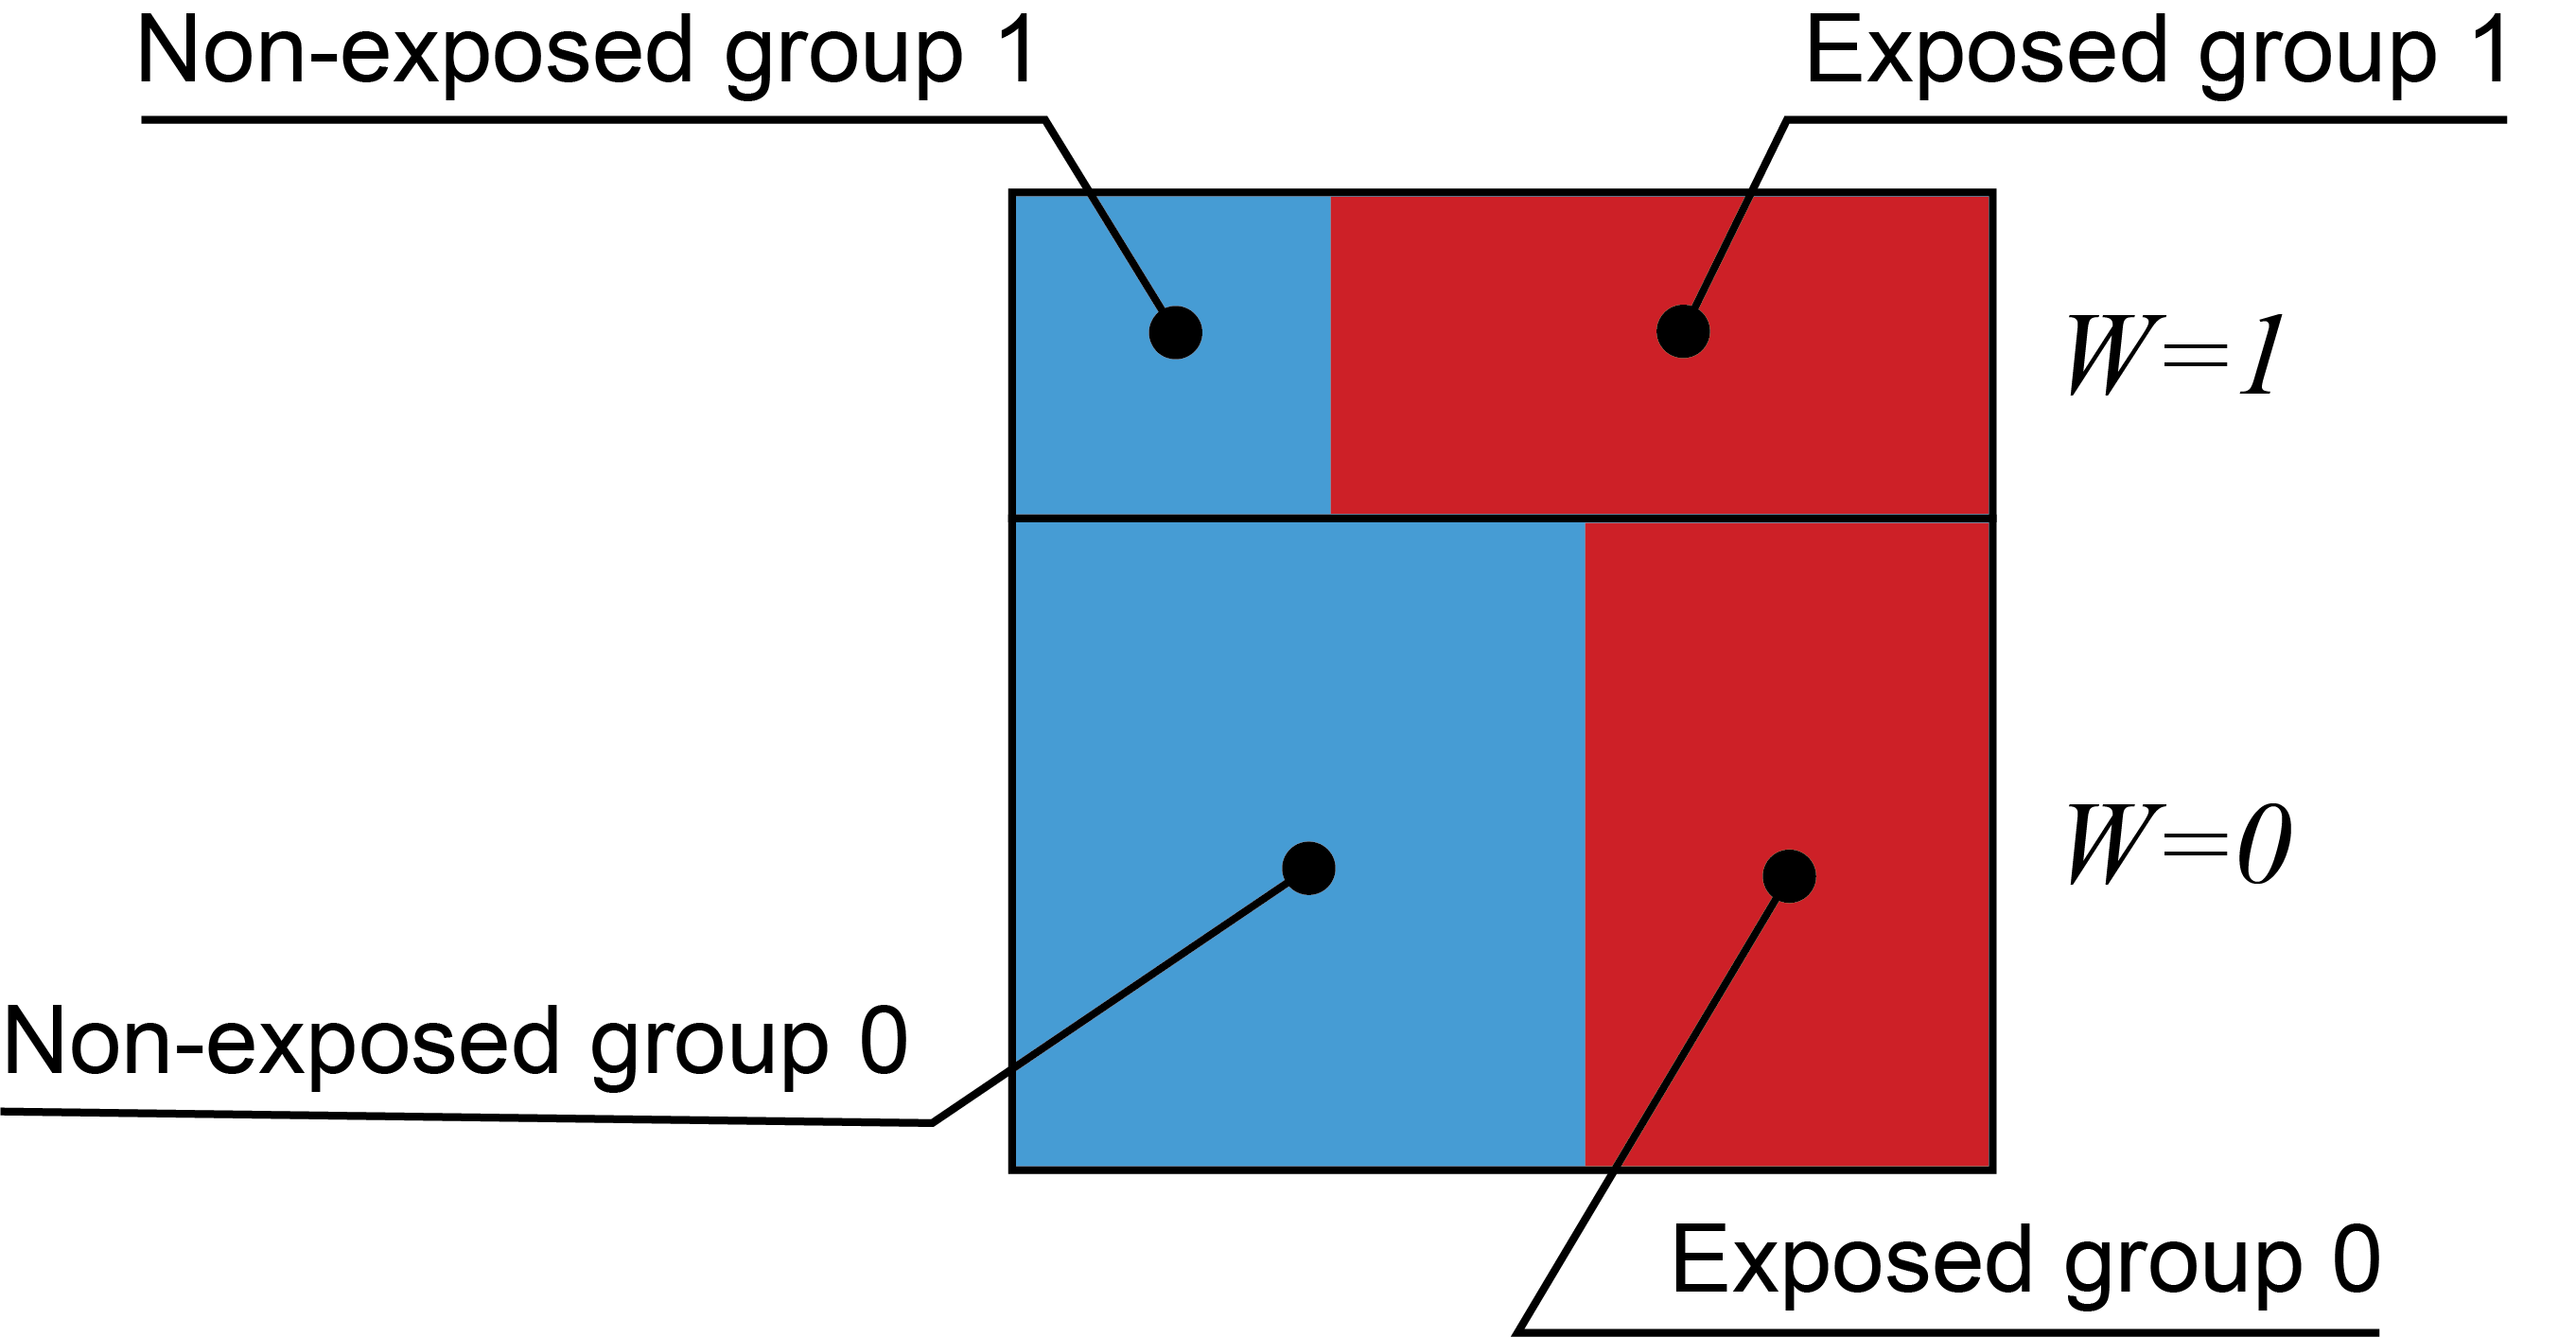
\includegraphics[width=0.85\linewidth]{images/block_diagram.png}
	\end{center}
\end{frame}

\begin{frame}{Causal Effects}
	Will define causal effects using potential outcomes
	~\\~\\
	\begin{equation*}
		\Large
		\eqnmarkbox[blue]{node0}{Y}^{\eqnmarkbox[red]{node1}{a}}_{\eqnmarkbox[darkgreen]{node2}{i}}
	\end{equation*}
	\annotate[yshift=1.25em]{above,left}{node0}{Outcome... }	
	\annotate[yshift=0.75em]{above,right}{node1}{...under a specific exposure...}	
	\annotate[yshift=-0.25em]{below,left}{node2}{...for a specific person}	
	~\\~\\
	For a binary exposure $A$, we can think of each person have two potential outcomes
	\begin{itemize}
		\item Potential outcome under exposure $Y^1$
		\item Potential outcome under non-exposure $Y^0$
	\end{itemize}
	~\\
	So causal effects are defined as contrasts of potential outcome
\end{frame}

\begin{frame}{Average Causal Effect -- Definition}
	One of the more well-known estimands from causal inference
	$$ E[Y_i^0] - E[Y_i^1] $$
	where $E[\cdot]$ is the expected value function\footnote[frame]{which you can think about as $1/n \sum_i^n (\cdot)$. Also $E[X] = \Pr(X=1)$ when $X$ is binary}
	~\\~\\
	Contrasts when every person \textit{is not exposed} versus when every person \textit{is exposed}
	\begin{itemize}
		\item This is implicitly what trials estimate
	\end{itemize}
\end{frame}

\begin{frame}{Average Causal Effect -- Diagram}
	\begin{center}
		
\includegraphics[width=0.85\linewidth]{images/ace.png}
	\end{center}
\end{frame}

\begin{frame}{Average Causal Effect -- Limitations}
	The average causal effect may not always be helpful for policy making
	~\\~\\
	Consider tobacco use:
	\begin{itemize}
		\item Scenario where everyone uses tobacco is unlikely to be useful
	\end{itemize}
	~\\
	Potential outcomes can be used to define other policies
\end{frame}

\begin{frame}{Natural Course}
	\begin{columns}
		\begin{column}{0.5\textwidth}
			To help define additional estimands, we introduce the \textit{natural course}\footnote[frame]{Rudolph et al. \textit{Am J Epidemiol} 2022; 191(2):341-348}
			$$ E \left[ Y_i^{A_i} \right] = E \left[Y_i \right] $$
			or the outcomes under the exposure distribution as observed
			\begin{itemize}
				\item The population as it is
			\end{itemize}
		\end{column}
		\begin{column}{0.5\textwidth}
			\centering
			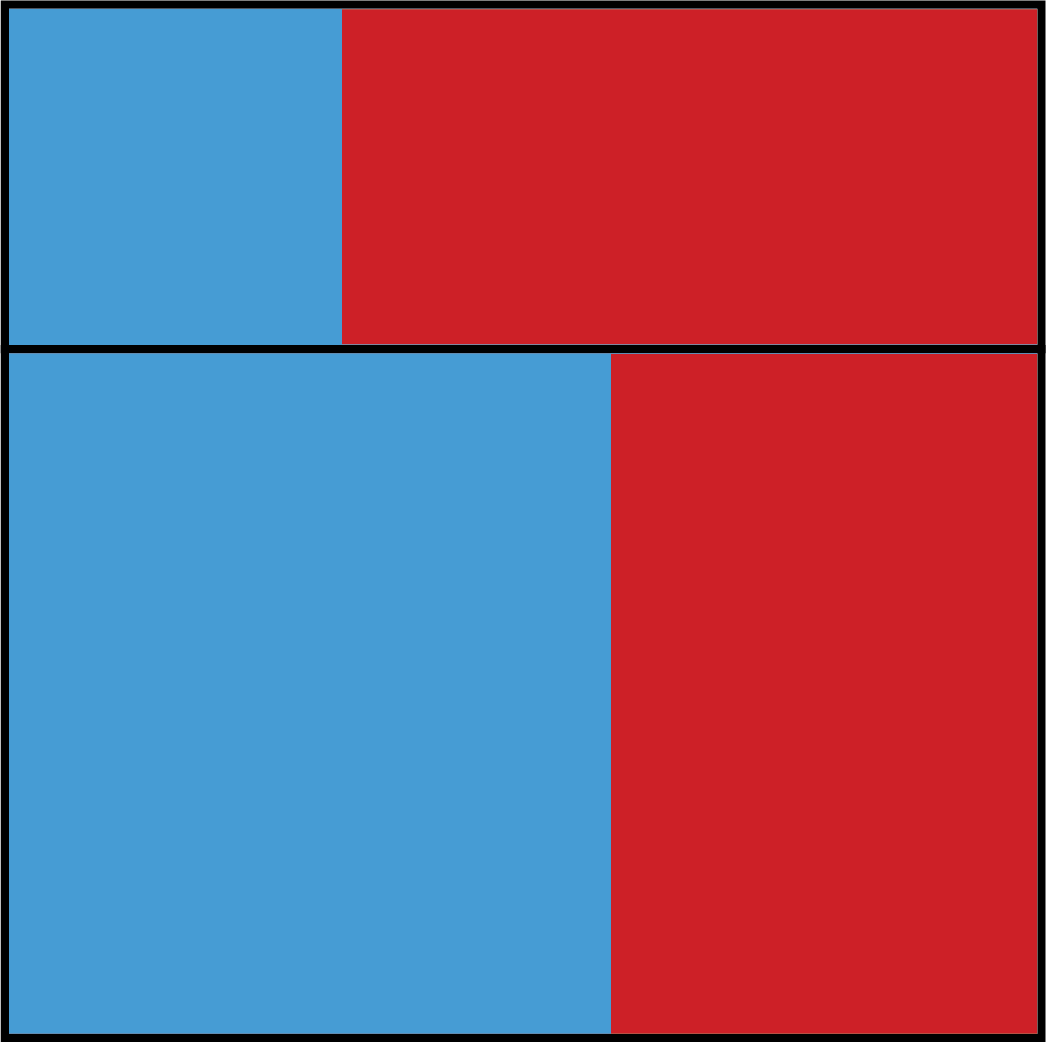
\includegraphics[width=0.8\linewidth]{images/natural_course.png}
		\end{column}
	\end{columns}
\end{frame}

\begin{frame}{Removing an Exposure -- Definition}
	Rather than force everyone to be exposed, can compare removal of an exposure\footnote[frame]{In the literature, these have been referred to as `population attributable' effects \\ Westreich \textit{Epidemiol} 2017; 28(4):525-528}
	$$ E[Y^0] - E[Y] $$
	~\\
	This comparison may have greater utility for harmful exposures
	\begin{itemize}
		\item Ex: reduction in outcome if eliminated all smoking
	\end{itemize}
\end{frame}

\begin{frame}{Removing an Exposure -- Diagram}
	\begin{center}
		
\includegraphics[width=0.85\linewidth]{images/abe.png}
	\end{center}
\end{frame}

%\begin{frame}{Selectively Removing an Exposure}
%	\begin{center}
%		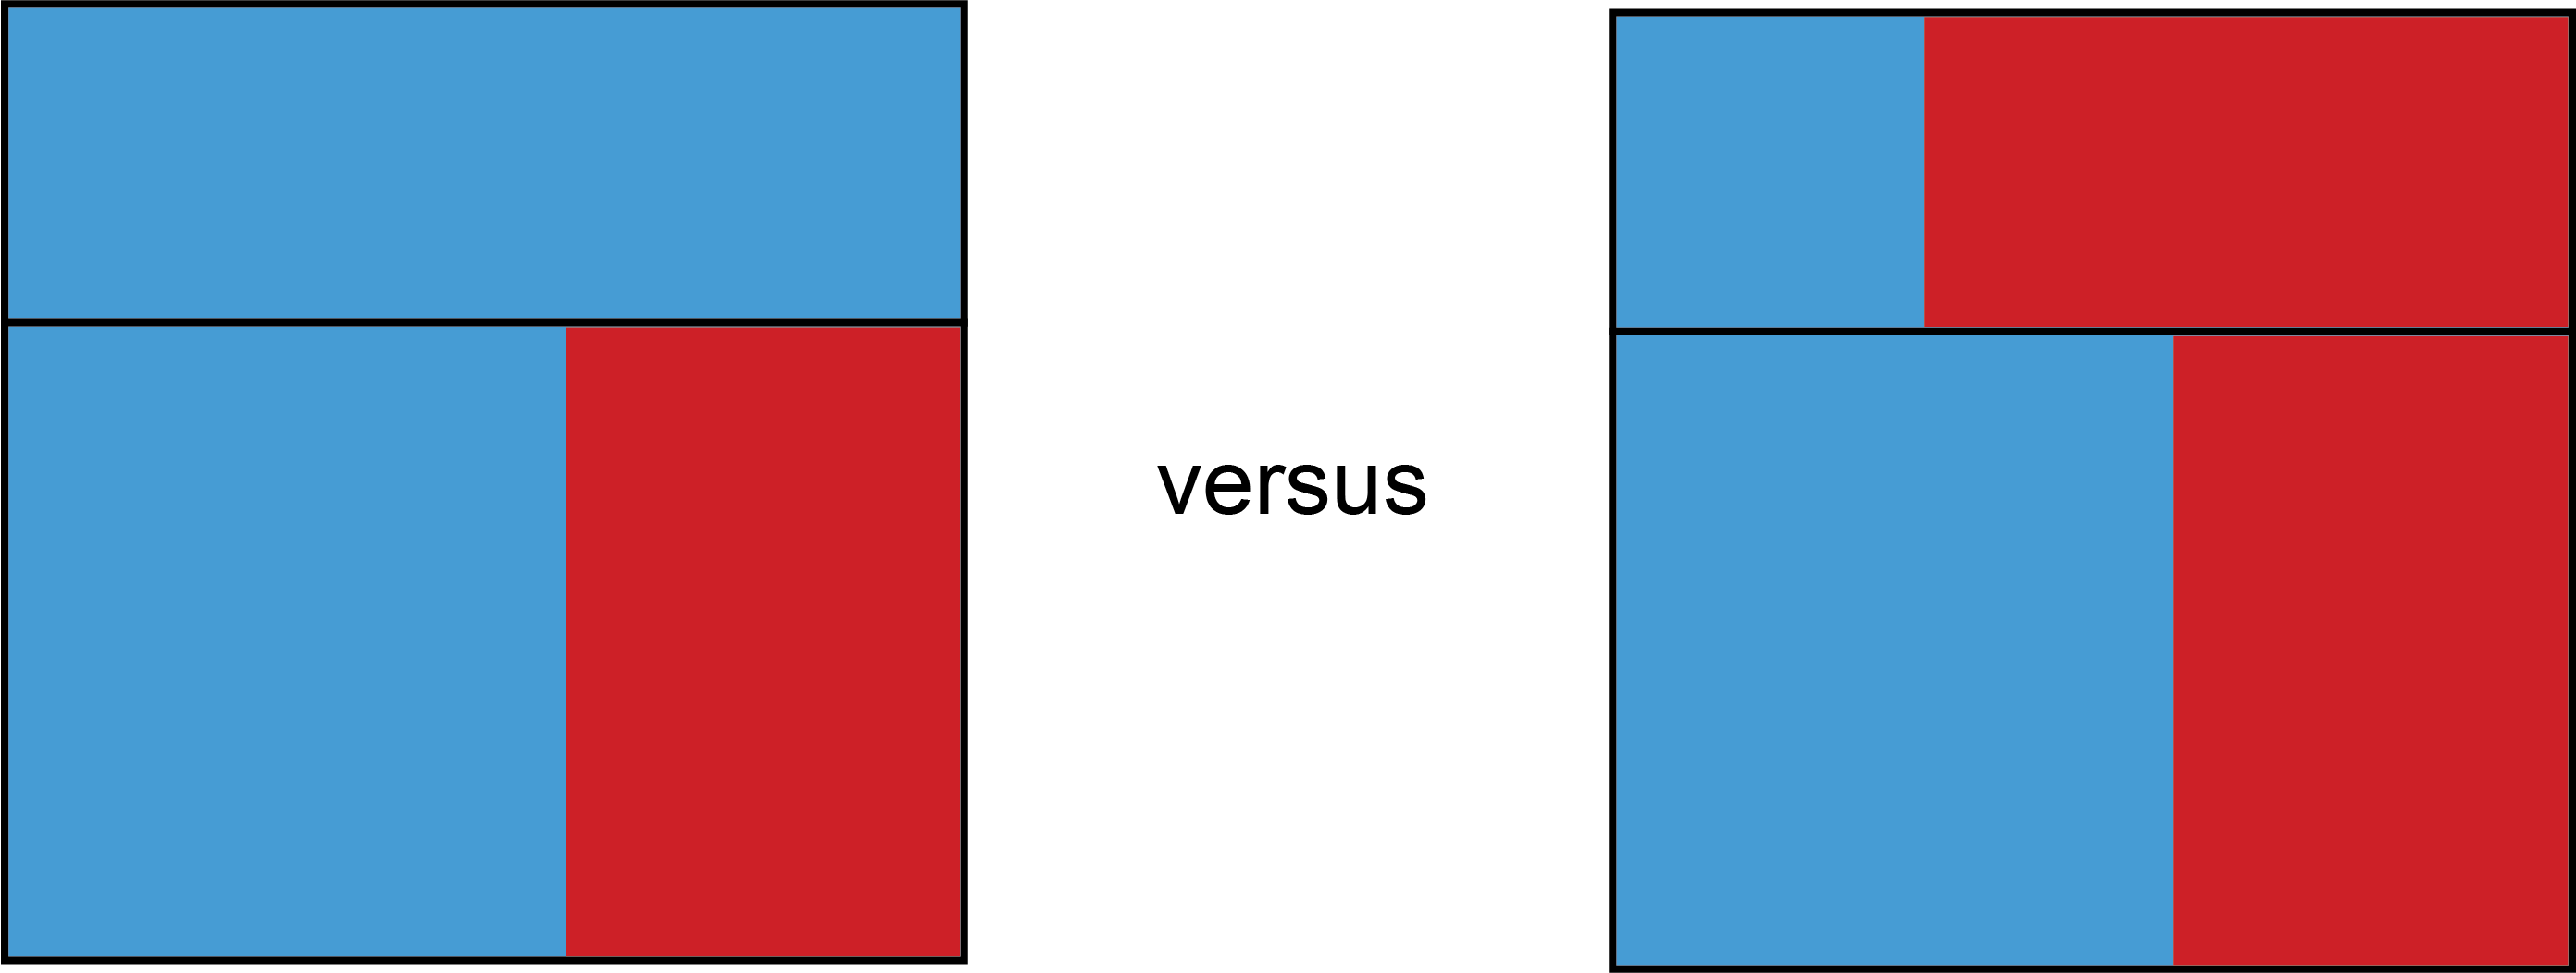
\includegraphics[width=0.85\linewidth]{images/sabe.png}
%	\end{center}
%\end{frame}

\begin{frame}{Reducing Exposure -- Definition}
	Removing an exposure completely is often overly optimistic
	\begin{itemize}
		\item Preventing \textit{all} tobacco smoking is not currently feasible
	\end{itemize}
	~\\
	Rather than \textit{deterministic} changes in exposure, we can consider changes in the \textit{probability} of exposure
	\begin{equation*}
		\left( \sum_{a \in \{0,1\}} E[Y^a] \times {\Pr}^*(A=a) \right) - E[Y]
	\end{equation*}
	where ${\Pr}^*$ denotes this is specified by the researcher
\end{frame}

\begin{frame}{Reducing Exposure -- Definition}
	For our binary $A$, this can also be written as
	\begin{equation*}
		\left( E[Y^1] \times {\Pr}^*(A=1) + E[Y^0] \times {\Pr}^*(A=0) \right) - E[Y]
	\end{equation*}
	~\\
	so think about this estimand as a weighted average of the mean potential outcomes, where the weights are the specified policy\footnote[frame]{Note that the removal of an exposure is the special case where ${\Pr}^*(A=0) = 1$}
\end{frame}

\begin{frame}{Reducing Exposure -- Diagram}
	\begin{center}
		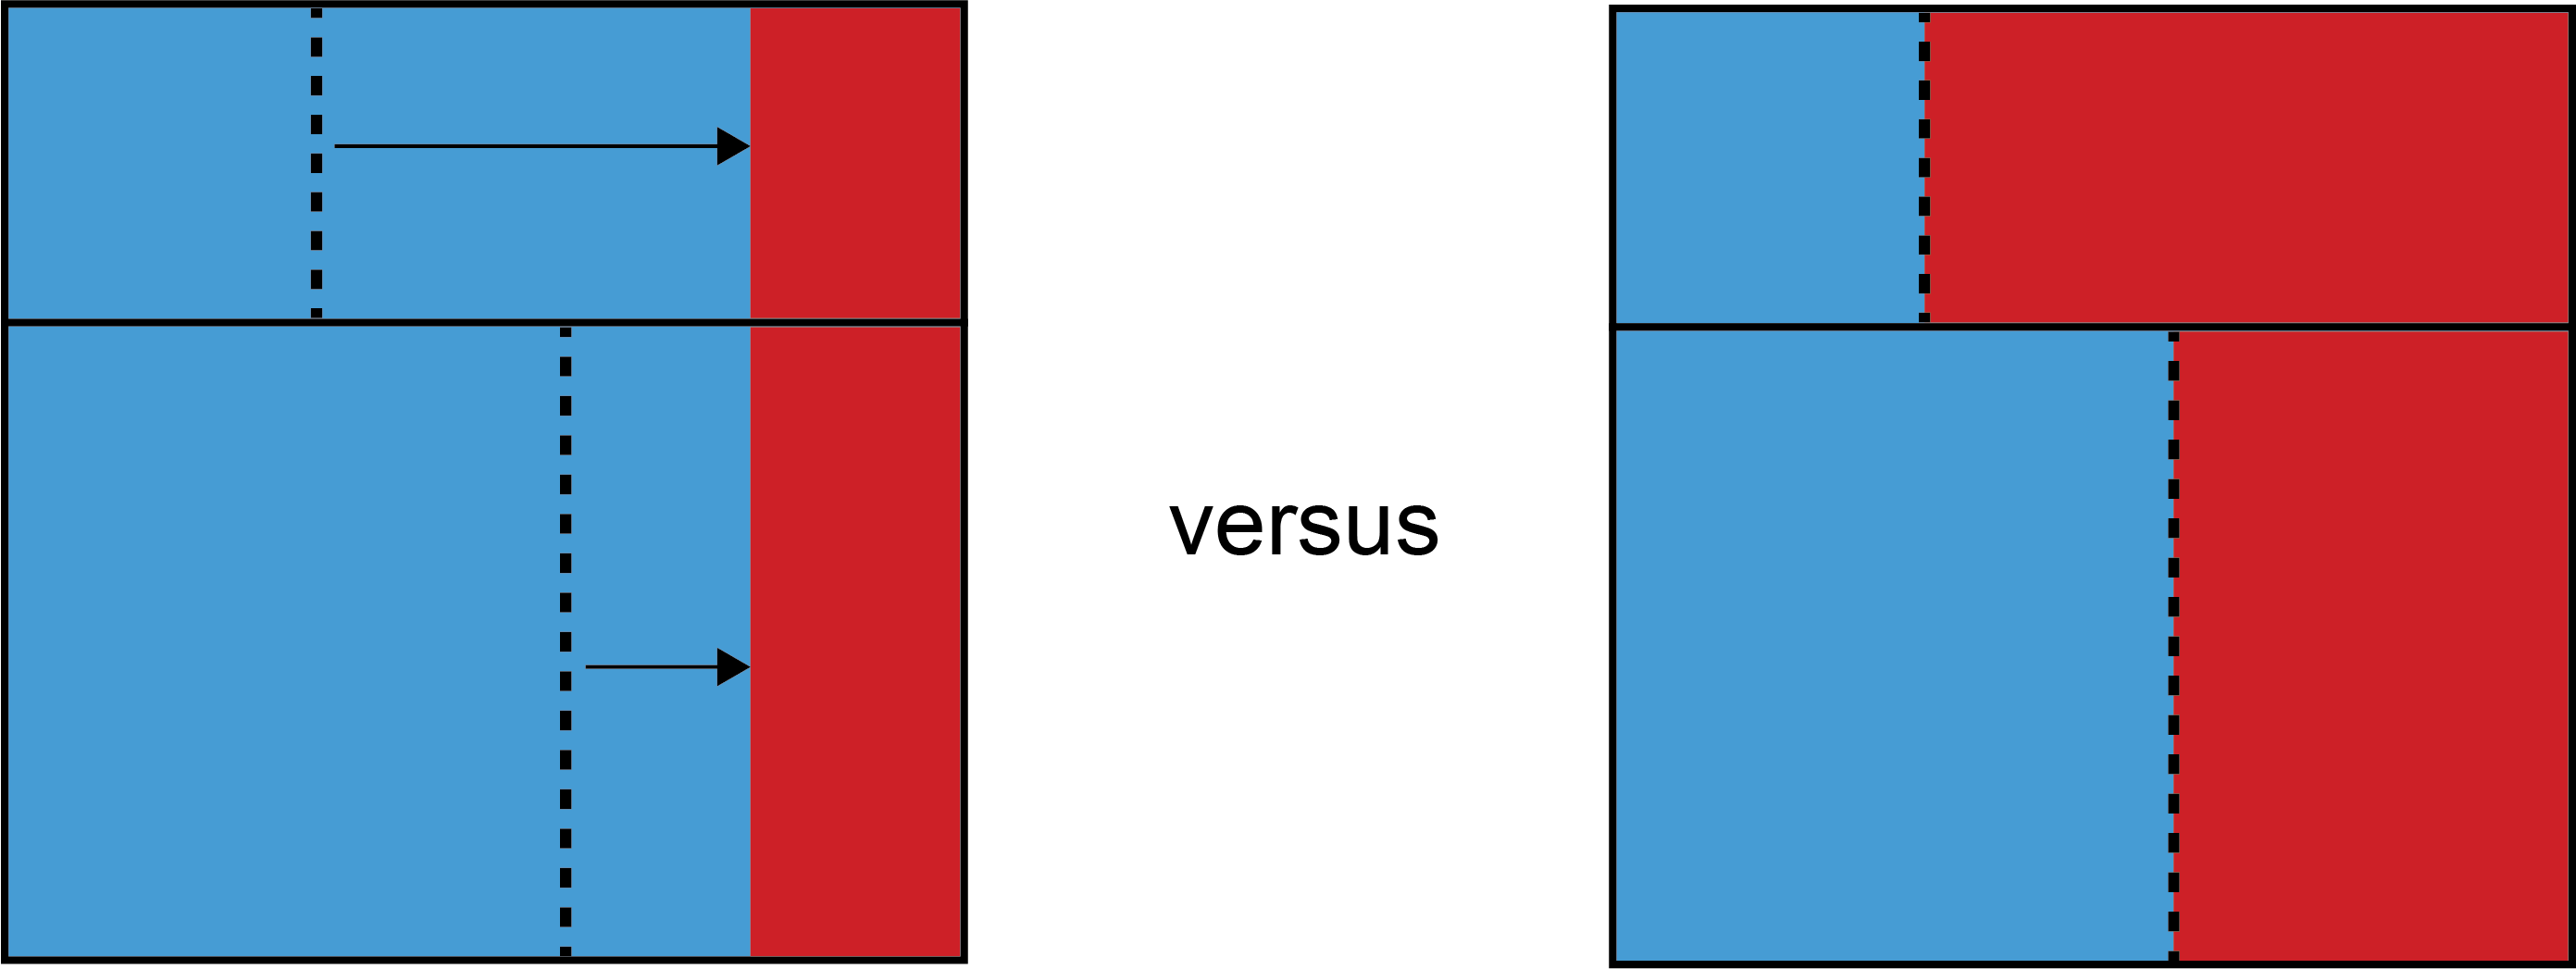
\includegraphics[width=0.85\linewidth]{images/stochastic.png}
	\end{center}
\end{frame}

\begin{frame}{Conditional Reductions -- Definition}
	Rather than set everyone to have the same probability of exposure, we can also modify the probability of exposure by $W$
	$$ E \left[ \sum_{a \in \{0,1\}} Y^a \times {\Pr}^*(A=a \mid W) \right] - E[Y] $$
	where the policy now incorporates $W$.\footnote[frame]{Incremental propensity score effects are one example \\ Naimi et al. \textit{Epidemiol} 2021:32(2):202-208}
	~\\~\\
	Study policies that differ in effectiveness of changing exposures by groups
	\begin{itemize}
		\item A smoking cessation program may be more effective in women relative to men
	\end{itemize}
\end{frame}

\begin{frame}{Conditionally Reductions -- Diagram}
	\begin{center}
		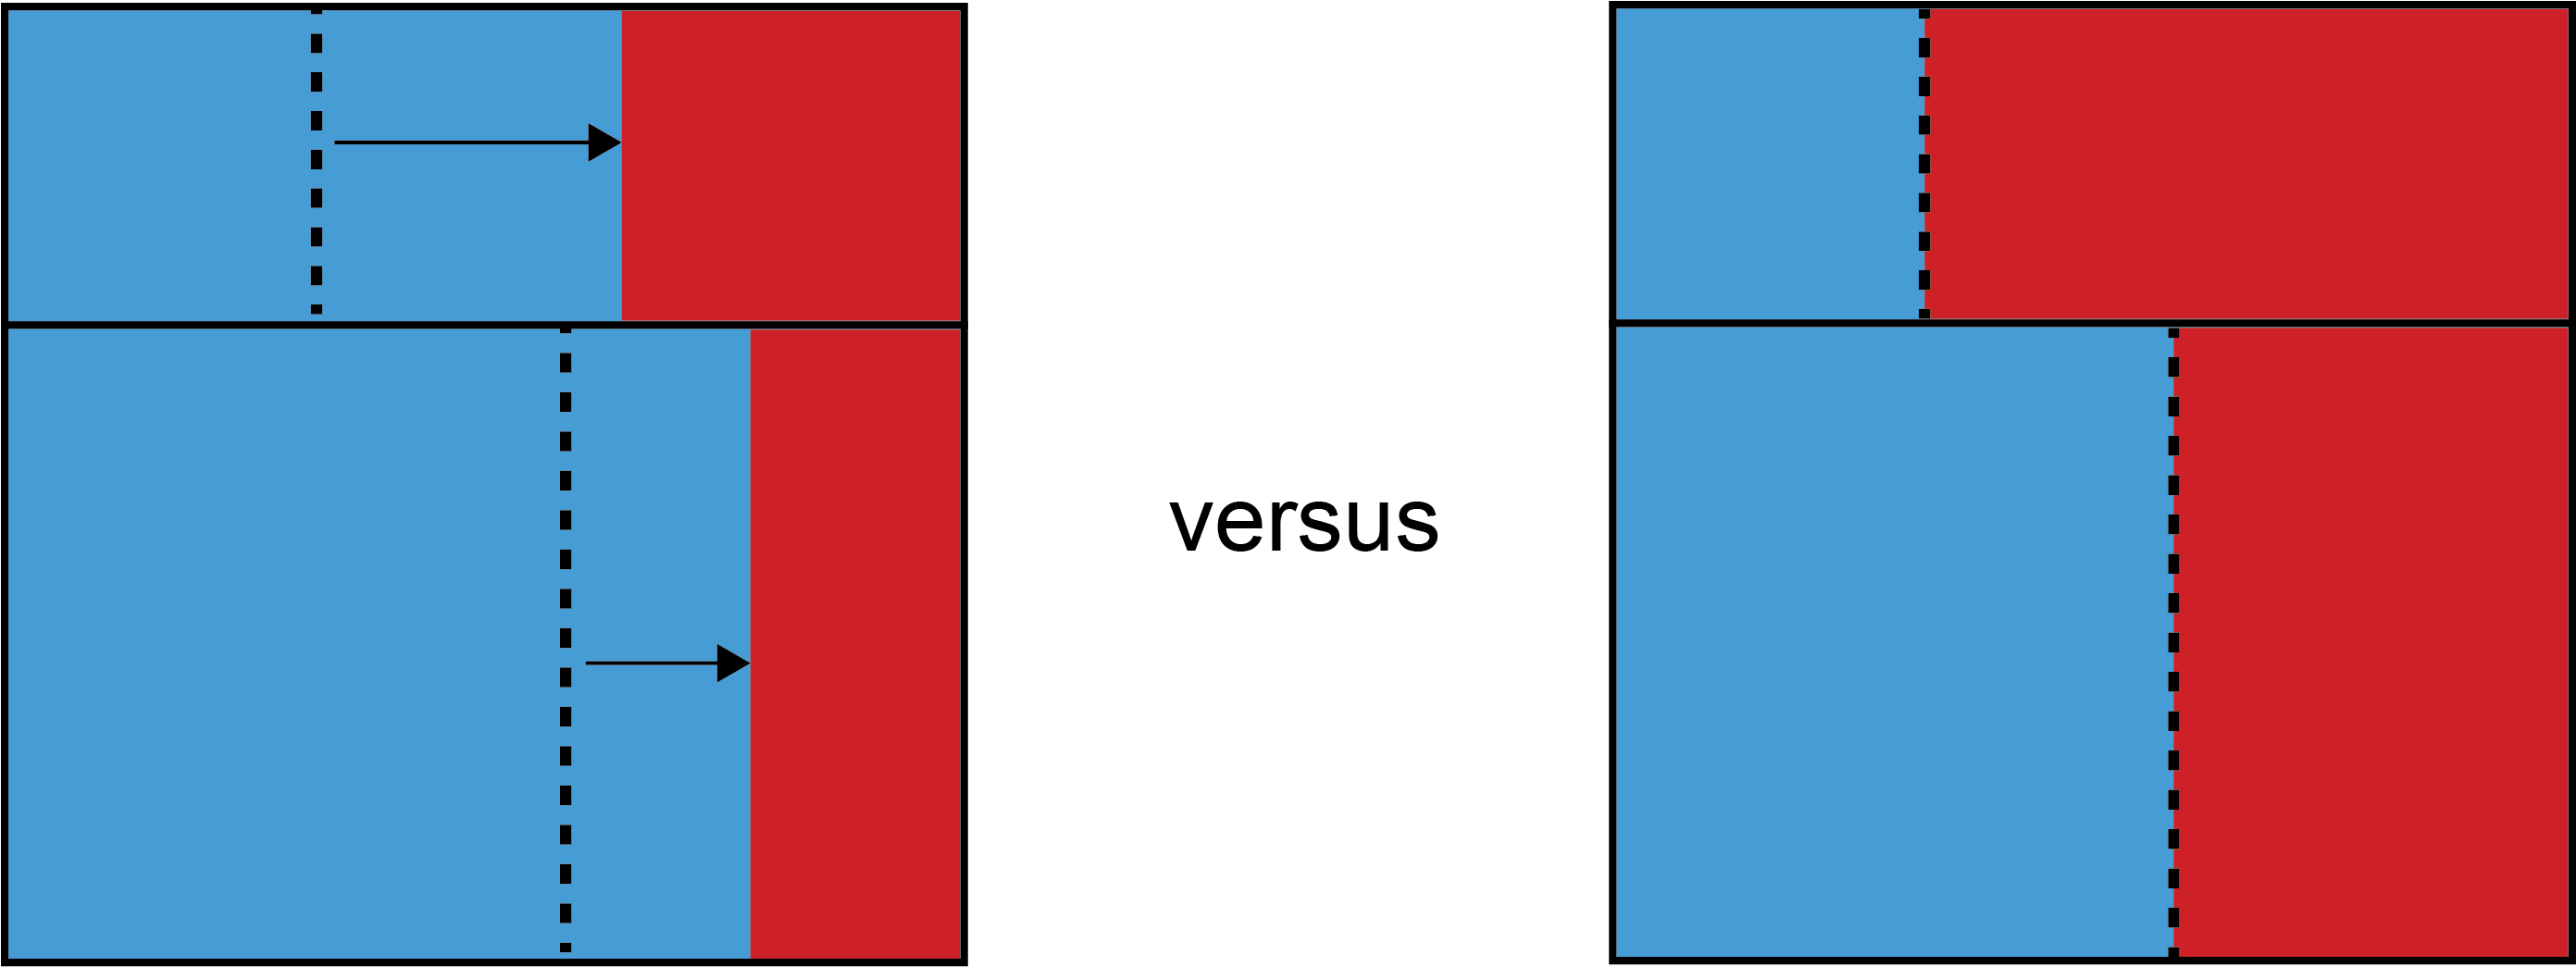
\includegraphics[width=0.85\linewidth]{images/stochastic_cond.png}
	\end{center}
\end{frame}

\begin{frame}{Comparing Exposure Reductions -- Definition}
	Rather than compare to the natural course, can directly compare competing policies
	$$ E \left[ \sum_{a \in \{0,1\}} Y^a \times {\Pr}^*(A=a \mid W) \right] - E \left[ \sum_{a \in \{0,1\}} Y^a \times {\Pr}^\#(A=a \mid W) \right] $$
	~\\
	For example, is it more effective to (1) greatly reduce exposure in one high-risk group, or (2) moderately reduce exposure across the population\footnote[frame]{Drawing inspiration from Rose \textit{Int J Epidemiol} 2001; 30(3):427-432}
\end{frame}

\begin{frame}{Comparing Exposure Reductions -- Diagram}
	\begin{center}
		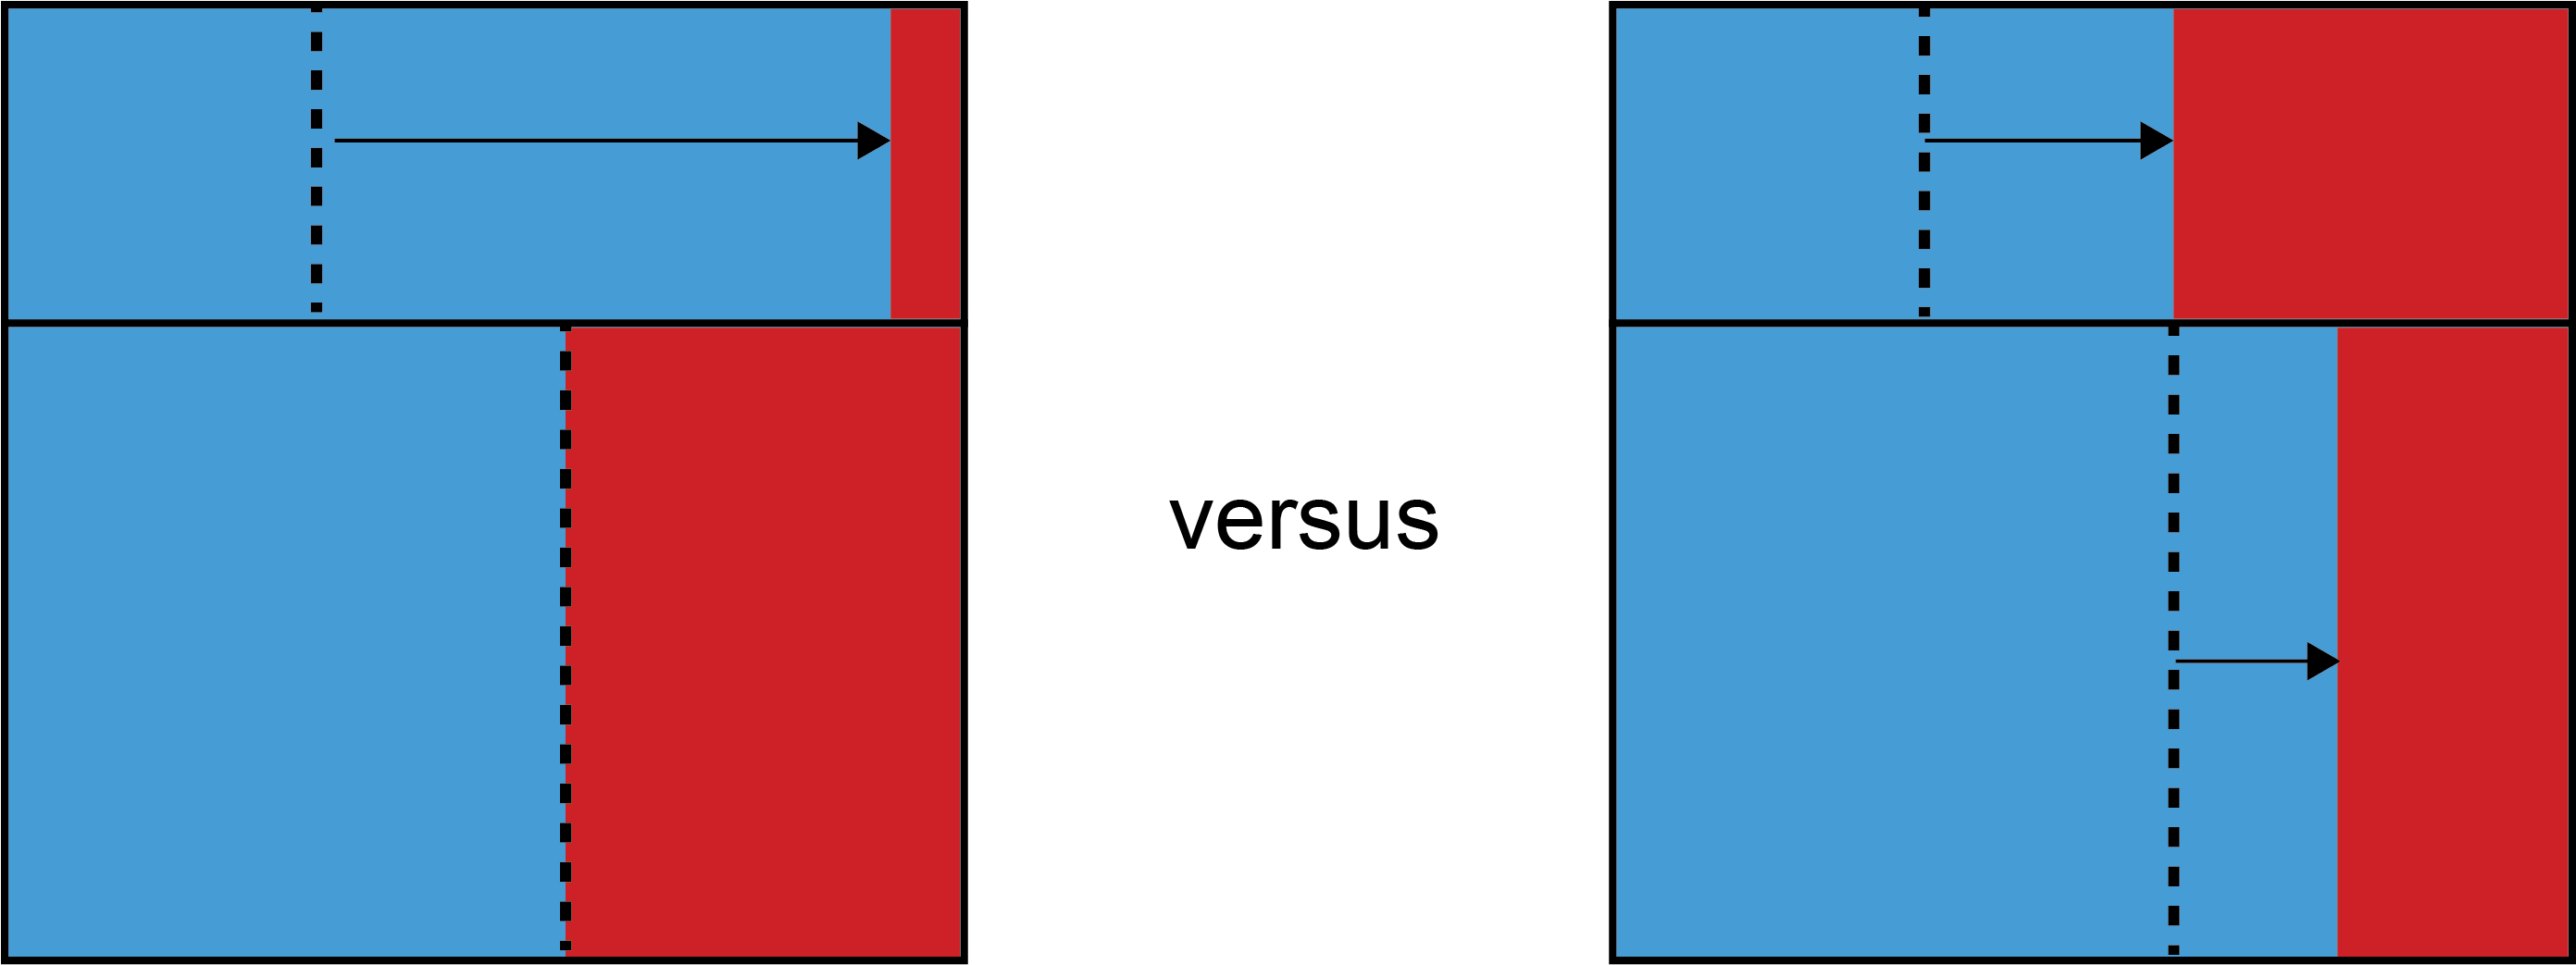
\includegraphics[width=0.85\linewidth]{images/stochastic_vs.png}
	\end{center}
\end{frame}

\begin{frame}{A Unified Expression for Policies}
	All the previous estimands can be expressed from the conditional reduction formula
	$$ E \left[ \sum_{a \in \{0,1\}} Y^a \times {\Pr}^*(A=a \mid W) \right] $$
	where each of the previous is a different specification for ${\Pr}^*(A=a \mid W)$
\end{frame}

\begin{frame}{Estimand Flow Diagram}
	\begin{center}
		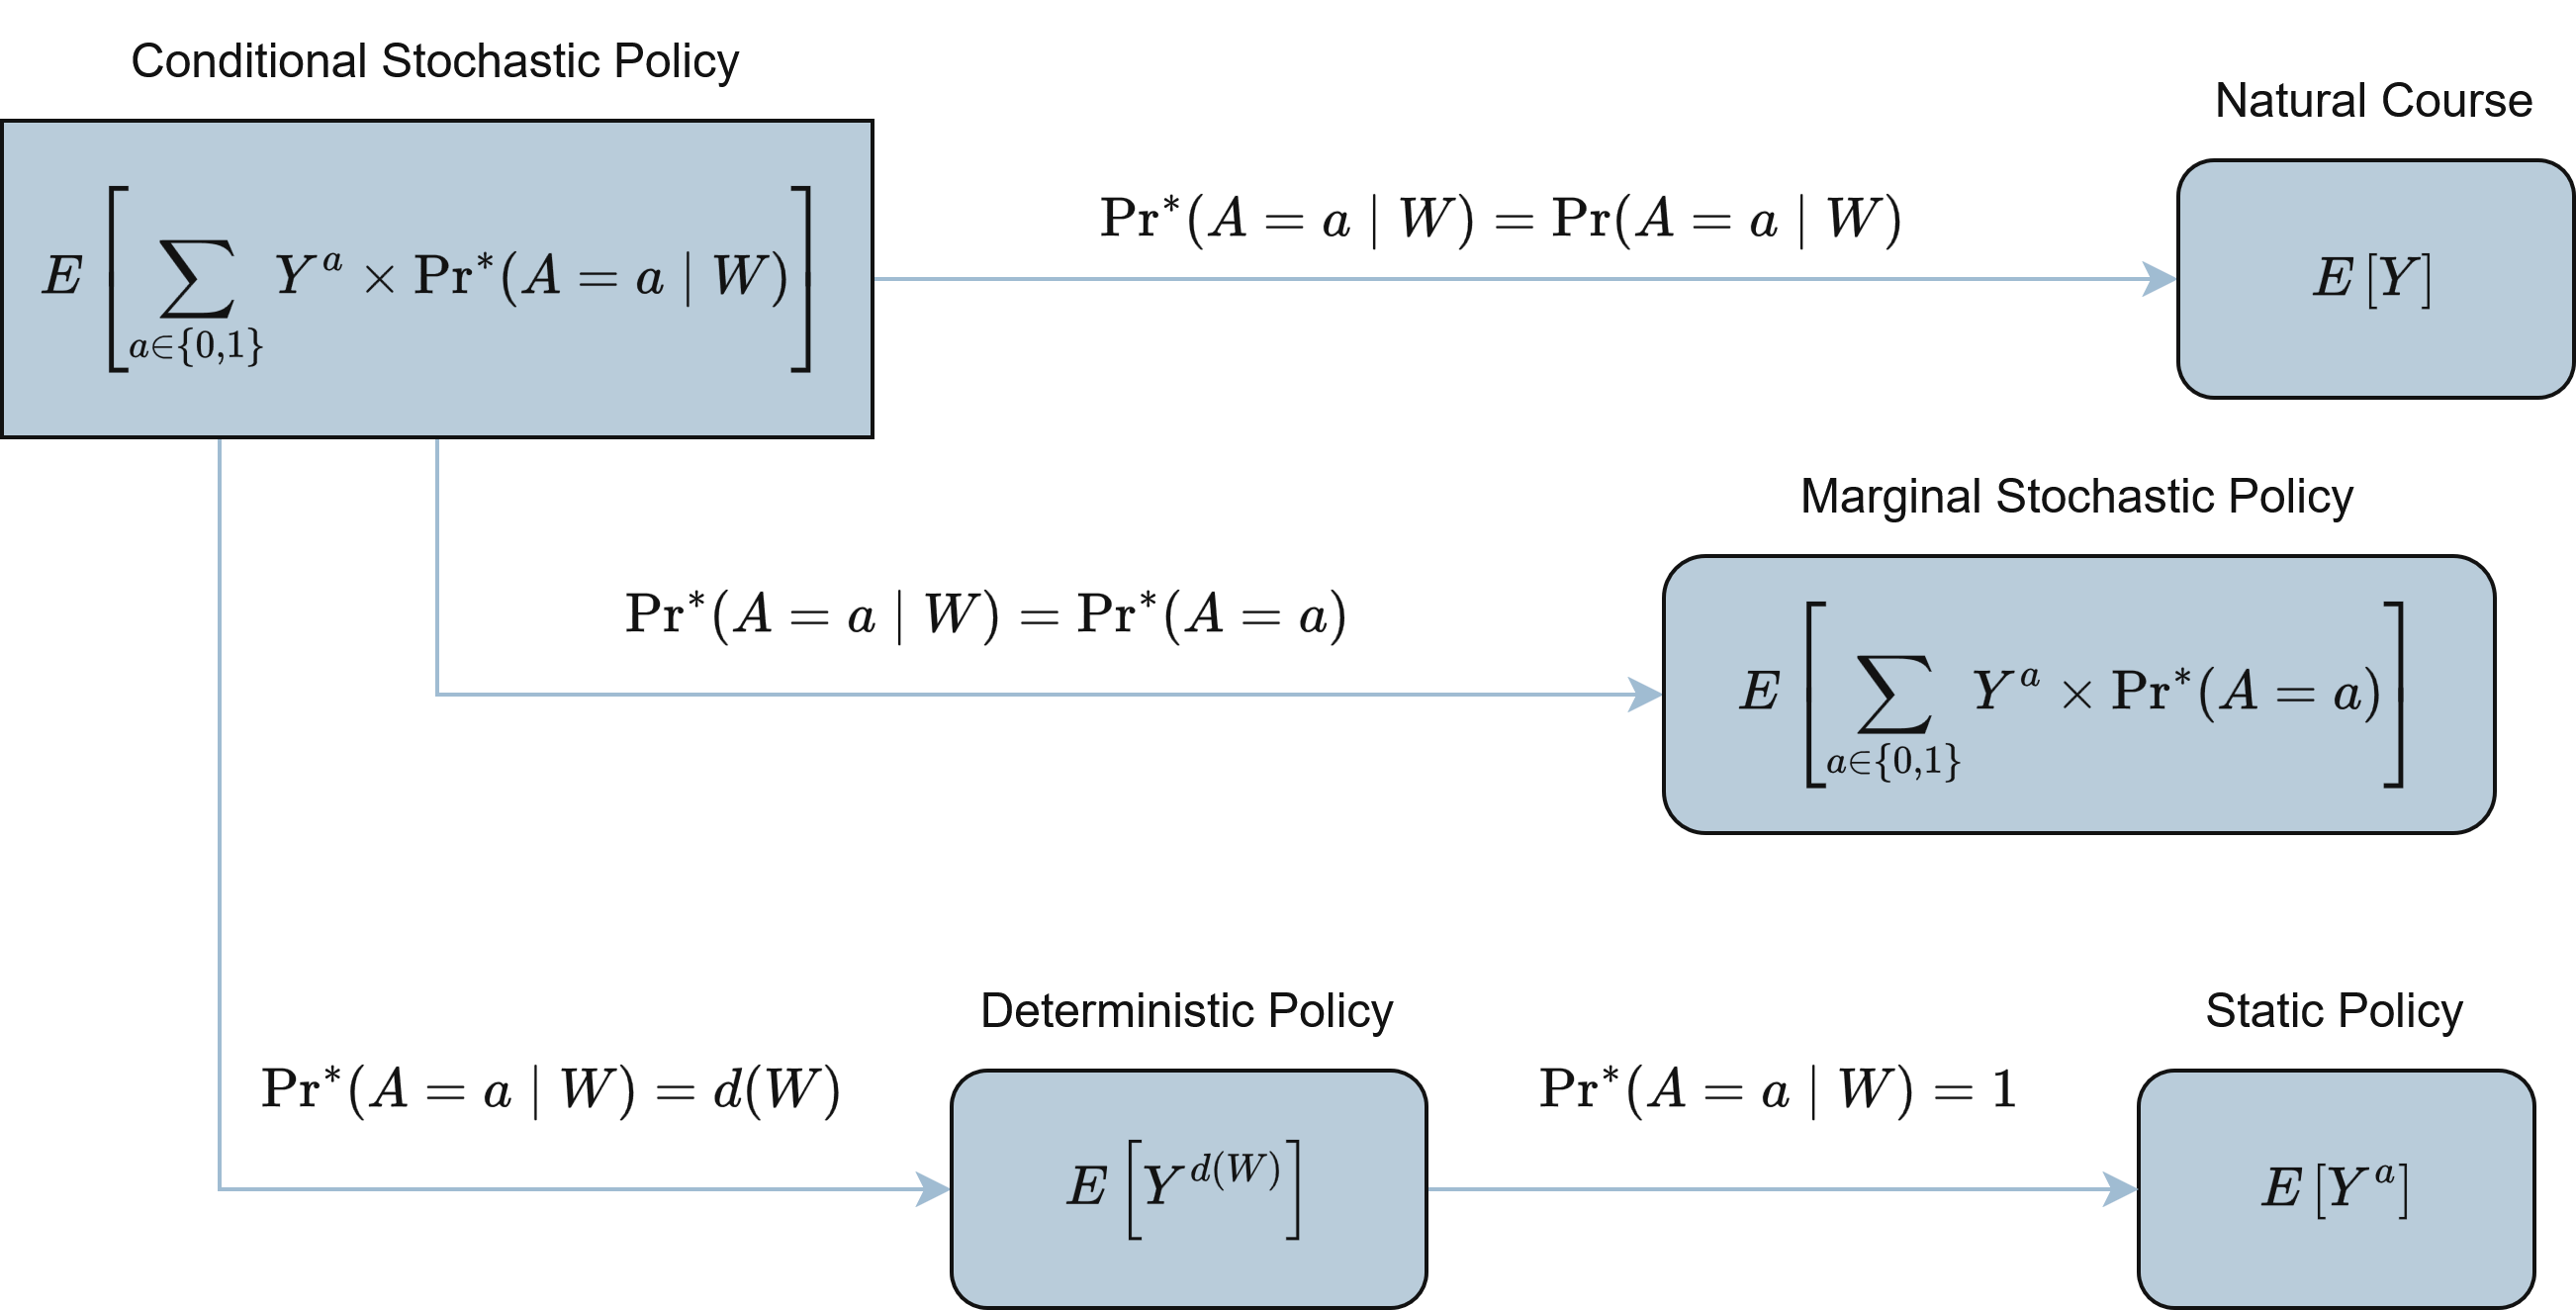
\includegraphics[width=0.85\linewidth]{images/schematic.drawio.png}
	\end{center}
\end{frame}

\begin{frame}{Identification and Estimation}
	Previous result indicates that identification proceeds similarly for all estimands\footnote[frame]{In fact, identification for probabilistic policies can proceed under weaker assumptions relative to the average causal effect, since exchangeability and positivity may only need to hold for subsets of the covariate space}
	~\\~\\
	Estimation can also be done using g-computation,\footnote[frame]{Ahern et al. \textit{Am J Epidemiol} 2009; 169(9):1140-1147} or inverse probability weighting
	\begin{itemize}
		\item G-computation: set $A$ according to specified policy and apply as normal
		\item Inverse probability weighting: $$I(A=a)\frac{{\Pr}^*(A=a \mid W)}{\Pr(A=a \mid W)}$$
	\end{itemize}
\end{frame}

\begin{frame}{Conclusions}
	Potential outcomes aid in the mapping from a specific question to the mathematical machinery that allows for quantitative effect estimation
	\begin{itemize}
		\item Can help to ensure results provide utility for decision makers
	\end{itemize}
	~\\
	Offer the greatest utility when understand how policy acts on $A$, or ${\Pr}^*(A=a \mid W)$
	\begin{itemize}
		\item If estimating ${\Pr}^*(A=a \mid W)$ using another data source, need to be careful about transportability and appropriately estimating the variance\footnote[frame]{A data fusion perspective will probably be helpful here \\ Cole et al. \textit{Am J Epidemiol} 2023; 192(3):467-474}
	\end{itemize}
\end{frame}

\begin{frame}{Thank You!}
	\begin{center}
		\small
		\faEnvelope \quad pzivich@unc.edu \qquad \quad 
		\faGithub \quad pzivich \qquad \quad
		\faHashtag \quad pausalz@bsky.social
	\end{center}	
\end{frame}

\end{document}
